\section*{Bonus : Triangle dans un cercle}

$A$ et $B$ sont deux points d'un cercle de centre $O$, tel que $\widehat{AOB}=54\degree$

\begin{center}
	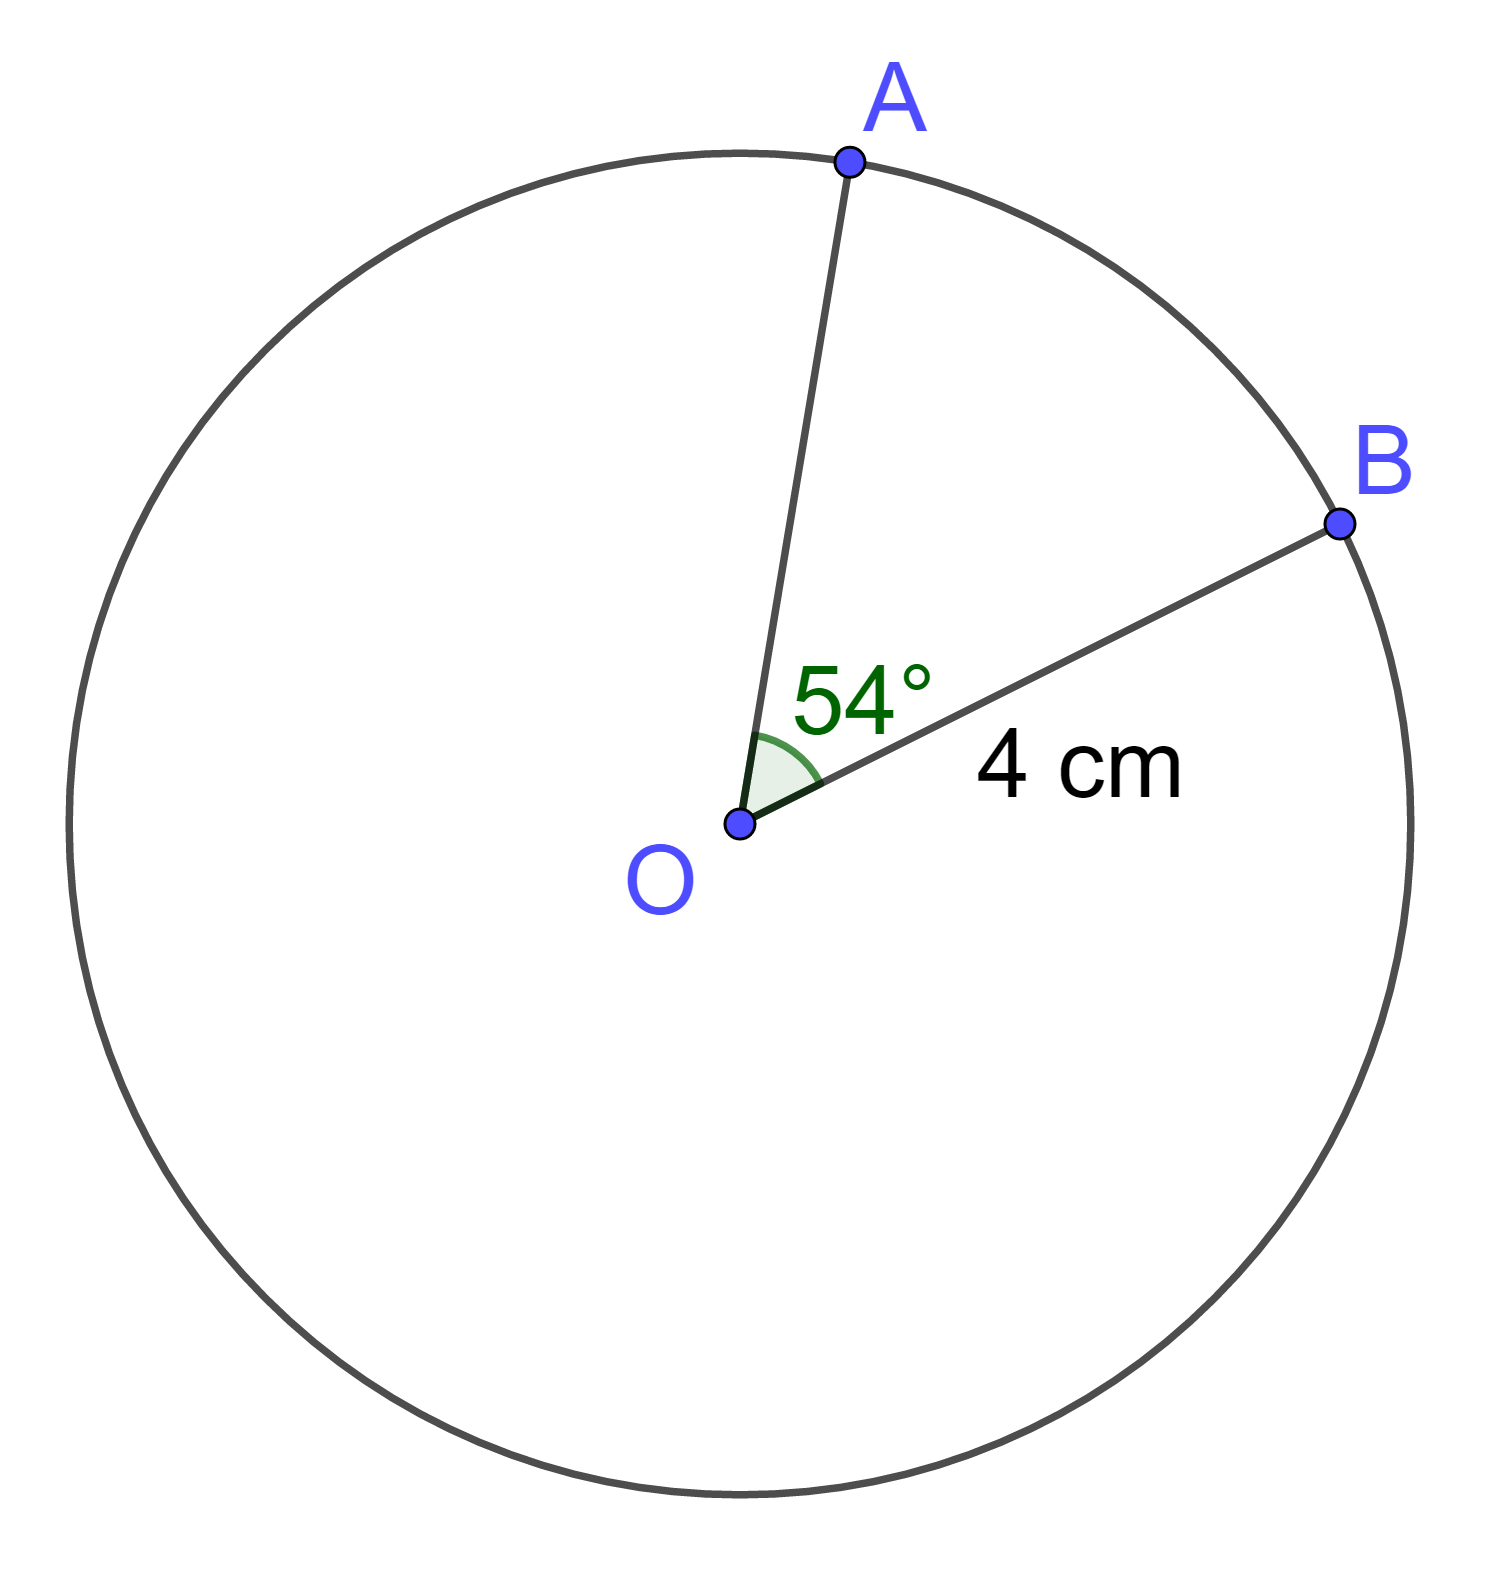
\includegraphics[scale=0.15]{img/cercle}
\end{center}

\begin{questions}
	\question Calculer la mesure de l'angle $\widehat{OAB}$. Expliquer la démarche et justifier.
\end{questions}
\begin{solution}
	$A$ et $B$ sont deux points d'un cercle de centre O. $[OA]$ et $[OB]$ sont des rayons de ce cercles, ils ont la même longueur. Donc le triangle $OAB$ est isocèle en $O$.
	
	Dans le triangle $OAB$ on a \monAngle{O} + \monAngle{A} + \monAngle{B} = 180\degree, et \monAngle{A} = \monAngle{B}.
	
	Dpnc : 
	
	\begin{eqnarray*}
		\widehat{A} &=& (180 - 54) \div 2\\
		\widehat{A} &=& 126 \div 2 \\
		\widehat{A} &=& 63 \\
	\end{eqnarray*}

Donc l'angle $\widehat{OAB}$ mesure 63\degree.
\end{solution}